\subsection{Analog til digital konvertering}
Mikrokontrolleren indeholder en SAR ADC, som gør det muligt at konvertere det analoge signal til et digitalt. Der ønskes at konfigurere 3 analoge kanaler, herunder Y-aksen på begge accelerometre samt EMG-måling. Opsætningen af ADC'en på mikrokontrolleren er illustreret på \autoref{fig:ADC_teori}. Der ønskes at læse signalerne hver for sig ved at måle single ended, hvorfor hvert input er koblet til $V_{ss}$.  Da der ønskes at anvende en 12 bit ADC, grundet kravet i \autoref{sec:ADC_teori}, indstilles denne til 12 bit, da der anvendes single ended svarer dette til at ADC'ens anvender 11 bit, hvorfor den inddeles i $2^{11}$ svarende til 2048 niveauer. ADC'en har et arbejdsområde fra $0-5~V$. LSB'en for ADC'en kan beregnes ud fra \autoref{equ:LSB}, hvilket giver $2,44~mV$, hvis denne overskrides vil den gå i mætning \citep{ADC2014}. 
\fxnote{Hvis der kobles flere til ting ADC'en skal dette skrives ind. Figuren er ikke endelig, så den skal udskiftes hvis det er.}
\begin{figure}[H]
\centering
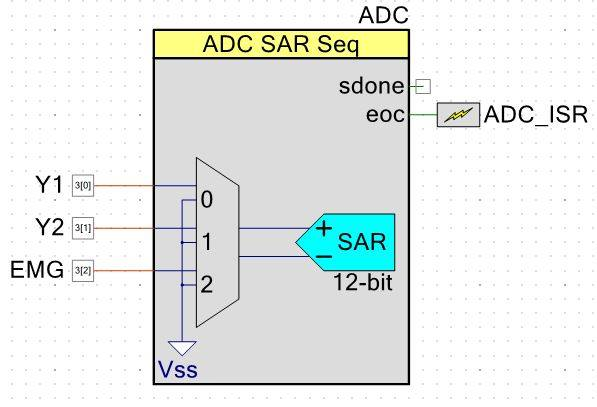
\includegraphics[width=1\textwidth]{figures/implementering/ADC_imp.png}
\caption{ADC'ens opsætning på mikrokontrolleren}
\label{fig:ADC_teori}
\end{figure}

I ADC'en er der indbygget en clock frekvens, da der ønskes at samples med 100 samples indstilles denne for at forholdet mellem clock frekvensen og samplingsfrekvensen er acceptabel(andet ord) skal samplingsfrekvens sættes til 101 samples per sekund, hvorved der opnås en hastighed på $1600~kHz$. 
